\documentclass[xcolor=dvipsnames,beamer]{beamer} %handout,notes=show

\usepackage{textcomp}
\usepackage[utf8]{inputenc}
% \usepackage{default}
\usepackage{graphicx}
%  \usepackage[pdftex]{hyperref}
\usepackage{url}
\usepackage{amsmath}

% frames have to be fragile
\newif\ifnotes
% \notestrue

%\notestrue


\ifnotes
%\setbeamertemplate{note page}[plain]
\setbeamertemplate{note page}[compress]
\setbeamerfont{note page}{size=\large}
\setbeameroption{show only notes}
%\setbeameroption{show notes}
\usepackage{pgfpages}
\pgfpagesuselayout{2 on 1}[a4paper,border shrink=5mm]%
\else
%\setbeameroption{hide notes}
\fi
%\notesfalse



% nastaveni TypeWriter
%\usepackage{courier}
%\usepackage{lmodern}
%\renewcommand*\ttdefault{txtt}
\DeclareFontShape{OT1}{cmtt}{bx}{n}{<5><6><7><8><9><10><10.95><12><14.4><17.28><20.74><24.88>cmttb10}{}


% \usepackage{verbatim}
\usepackage[absolute,overlay]{textpos}

\usepackage{listings}
% \usepackage{courier}
\definecolor{grey}{RGB}{70,70,70}
\definecolor{green}{RGB}{0,255,0}
\definecolor{red}{RGB}{202,53,53}
\definecolor{lightGrey}{RGB}{250,250,250}
\definecolor{darkGrey}{RGB}{50,50,50}


\usepackage{color}
\definecolor{lightgray}{rgb}{.9,.9,.9}
\definecolor{darkgray}{rgb}{.4,.4,.4}
\definecolor{purple}{rgb}{0.65, 0.12, 0.82}


% \usetheme{Warsaw}
\usetheme{Madrid}
% \usetheme{Szeged}
% \useoutertheme{infolines}
\usecolortheme[named=MidnightBlue]{structure}
% \usecolortheme[named=PineGreen]{structure}
% \setbeamertemplate{navigation symbols}{}




\title[HPC benchmarking ET models OSGEO]
{HPC benchmarking of ET models with OSGEO tools}
%\subtitle{SVO\v{C}}
%\pdforstring{}{}
\author[Yann Chemin]
{Yann Chemin}

\institute[IWMI]
{International Water Management Institute\\
\vspace{20pt}
% 
\includegraphics[width=1cm]{iwmi}
}
\date{April 11, 2013}


%\AtBeginSection[]{\begin{frame}\frametitle{Obsah}%
%\tableofcontents[currentsection ]\end{frame}}
%\AtBeginSubsection[]
%{
%  \begin{frame}<beamer>
%  \frametitle{Obsah}
%  \tableofcontents[currentsection,currentsubsection]
%  \end{frame}
%}

\setbeamercovered{transparent}

\hypersetup{%
	pdfauthor={Yann Chemin},%
	pdfsubject={Presentation},%
    pdfkeywords={HPC, benchmarking, Evapotranspiration, models, OSGEO}
}

\usepackage{listings}
\lstdefinestyle{C++}{%
  % language
  language=C++, % [ANSI]C++, GNU, ISO, Visual
  basicstyle=\ttfamily\small,
  commentstyle=\itshape,
  keywordstyle=\bfseries, % needs another \ttdefault
  showstringspaces=false,
  stringstyle=,
  identifierstyle=,
  % working with latex
  escapeinside={//lst}{\^^M}  
}

\lstset{%
%  frame=trBL,
%  backgroundcolor=\color{},
  linewidth=\textwidth,
  % working with latex
  gobble=2,
  % float
  nolol=false,
  numberbychapter=true,
  captionpos=t,% tb
  % breaking lines
  breaklines=true,
  breakatwhitespace=true,
  breakindent=10em,
  breakautoindent=true,
  prebreak={},
  postbreak={},
  %document default style
    basicstyle=\ttfamily
}


%\lstlistlistingname % The header name for the list of listings.
%\lstlistingname % The caption label for listings.

\lstnewenvironment{cmdline}[1][]
{\lstset{
  style=C++,
  #1}}
{}

\lstnewenvironment{scpp}[1][]
{\lstset{
  style=C++,
  #1}}
{}

\lstnewenvironment{ncpp}[1][]
{\lstset{
  style=C++,
  numbers=left, 
  numberstyle=\scriptsize, 
  stepnumber=1,
  numbersep=5pt,
  #1}}
{}

\lstnewenvironment{fcpp}[1][]
{\lstset{
  style=C++,
  float,
   % line numbers
  numbers=left, 
  numberstyle=\scriptsize, 
  stepnumber=1,
  numbersep=5pt,
  #1}}
{}


\lstnewenvironment{lcpp}[1][]
{\lstset{%
style=C++,
numbers=left, 
numberstyle=\scriptsize, 
stepnumber=1,
numbersep=5pt,
xleftmargin=12pt,
breakautoindent=false,
breaklines=false,%
#1}}{}

\lstnewenvironment{smallcpp}[1][]
{\lstset{%
style=C++,
numbers=left, 
numberstyle=\tiny, 
stepnumber=1,
numbersep=5pt,
xleftmargin=12pt,
breakautoindent=false,
breaklines=false,%
basicstyle=\ttfamily\scriptsize,
#1}}{}


\lstnewenvironment{pscpp}[1][]
{\lstset{%
style=C++,
xleftmargin=12pt,
breakautoindent=false,
breaklines=false,
#1}}{}


%\lstset{index={square},index={[2]root}}


\newcommand{\overovaciref}[1]{{\scriptsize(\ref{#1})}}


\usepackage{tipa}
\newcommand{\pron}[2]{#1 [#2]}

%%%%%%%%%%%%%%%%%%%%%%%%%%%%%%%%%%%%%%%%%%%%%%%%%%%%%%%%%%%%%%%%%%%%
%%%%%%%%%%%%%%%%%%%%%%%%%%%%%%%%%%%%%%%%%%%%%%%%%%%%%%%%%%%%%%%%%%%%
%%%%%%%%%%%%%%%%%%%%%%%%%%%%%%%%%%%%%%%%%%%%%%%%%%%%%%%%%%%%%%%%%%%%
%%%%%%%%%%%%%%%%%%%%%%%%%%%%%%%%%%%%%%%%%%%%%%%%%%%%%%%%%%%%%%%%%%%%
\begin{document}
%%%%%%%%%%%%%%%%%%%%%%%%%%%%%%%%%%%%%%%%%%%%%%%%%%%%%%%%%%%%%%%%%%%%
\frame{
\titlepage
}
%%%%%%%%%%%%%%%%%%%%%%%%%%%%%%%%%%%%%%%%%%%%%%%%%%%%%%%%%%%%%%%%%%%%%
\begin{frame}{Contents}
\tableofcontents
\end{frame}
%%%%%%%%%%%%%%%%%%%%%%%%%%%%%%%%%%%%%%%%%%%%%%%%%%%%%%%%%%%%%%%%%%%%

\section{Introduction}
%%%%%%%%%%%%%%%%%%%%%%%%%%%%%%%%%%%%%%%%%%%%%%%%%%%%%%%%%%%%%%%%%%%%
\begin{frame}[fragile]{Overview}

Evapotranspiration is the largest transiting quantity in the daily 
hydrological cycle along with rain. It is used by scientists and
managers in:
\newline\linebreak

\begin{itemize}
 \item Irrigation systems performance
 \item Crop water productivity
 \item Water accounting
 \item Wetlands-agriculture interface
 \item Basin water uses quantification
 \item Climate change on water cycle \& users
\end{itemize}


\end{frame}

\section{Evapotranspiration Modeling}
\subsection{Overview}
%%%%%%%%%%%%%%%%%%%%%%%%%%%%%%%%%%%%%%%%%%%%%%%%%%%%%%%%%%%%%%%%%%%%
\begin{frame}[fragile]{Overview}

There are several types of evapotranspiration modeling methods:\\

\begin{itemize}
 \item Reference ET: Hargreaves, Penman-Monteith
 \item Potential ET: Priestley-Taylor, astronomical
 \item Actual ET: Thermodynamic/energy balance (mostly)
\end{itemize}

\begin{block}{OSGEO tools}
\begin{columns}[l]
\column{0.2\textwidth}
\begin{center}

\includegraphics[width=2cm]{OSGeo_logo}
\end{center}
\column{0.4\textwidth}
\begin{center}
\includegraphics[width=2cm]{GDALLogoColor}
\end{center}
\column{0.4\textwidth}
\begin{center}

\includegraphics[width=2cm]{Grass_GIS}
\end{center}
\end{columns}
\end{block}
\end{frame}

\subsection{ET examples}
%%%%%%%%%%%%%%%%%%%%%%%%%%%%%%%%%%%%%%%%%%%%%%%%%%%%%%%%%%%%%%%%%%%%
\begin{frame}[fragile]{Evapotranspiration @ country level}

Actual evapotranspiration (365 days integrated)\\ 
for water resources monitoring \& management.\\

\begin{center}
 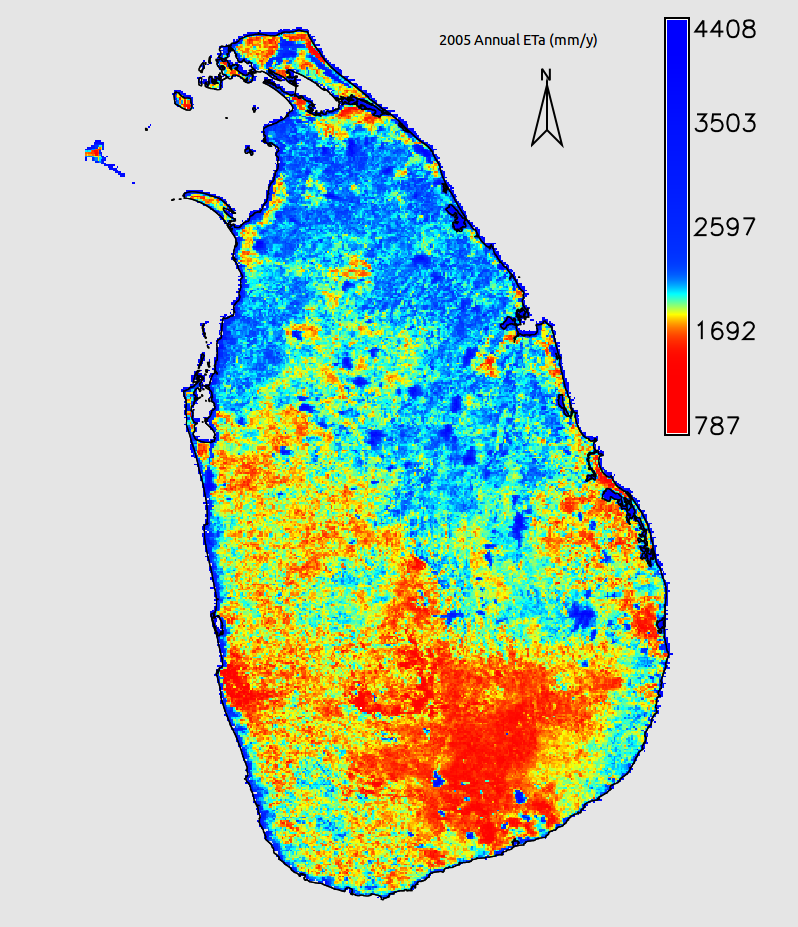
\includegraphics[width=5cm]{slet2005}
 \hspace{10mm}
 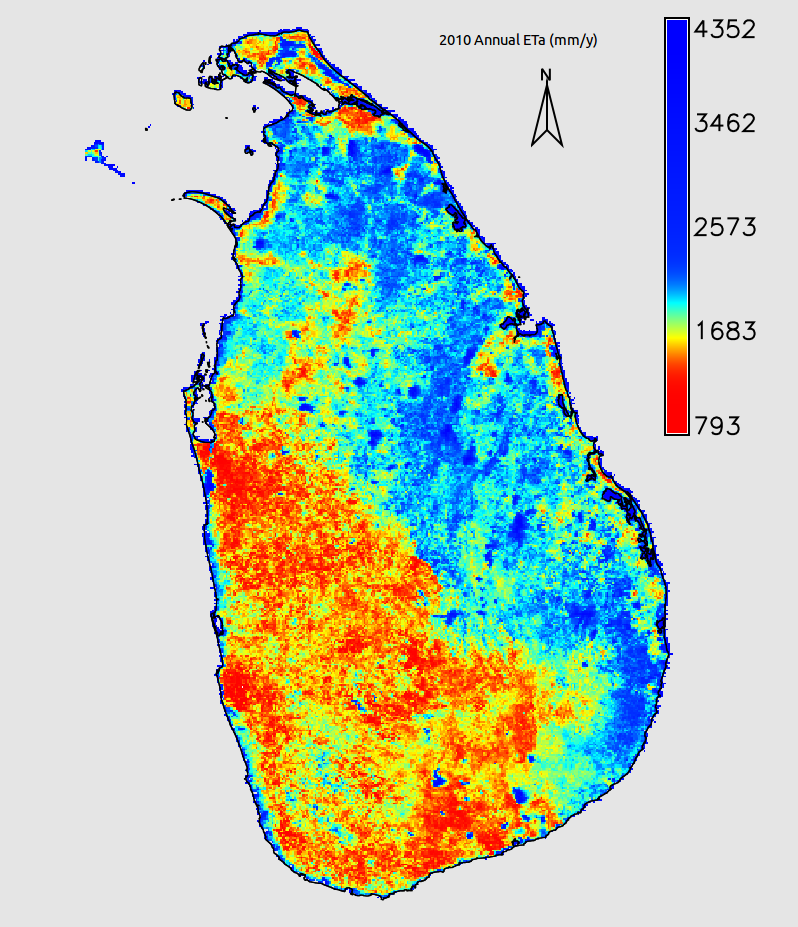
\includegraphics[width=5cm]{slet2010}
\end{center}

\end{frame}

%%%%%%%%%%%%%%%%%%%%%%%%%%%%%%%%%%%%%%%%%%%%%%%%%%%%%%%%%%%%%%%%%%%%
\begin{frame}[fragile]{Equity of water use in irrigation systems}

Irrigation water monitoring \& management
\begin{itemize}
 \item Map: Uniform colour is equity of water distribution
 \item Graph: irrigation system equity in time (mm/d, daily, 12 years)
\end{itemize}

\begin{columns}[l]
\column{0.2\textwidth}
\begin{center}
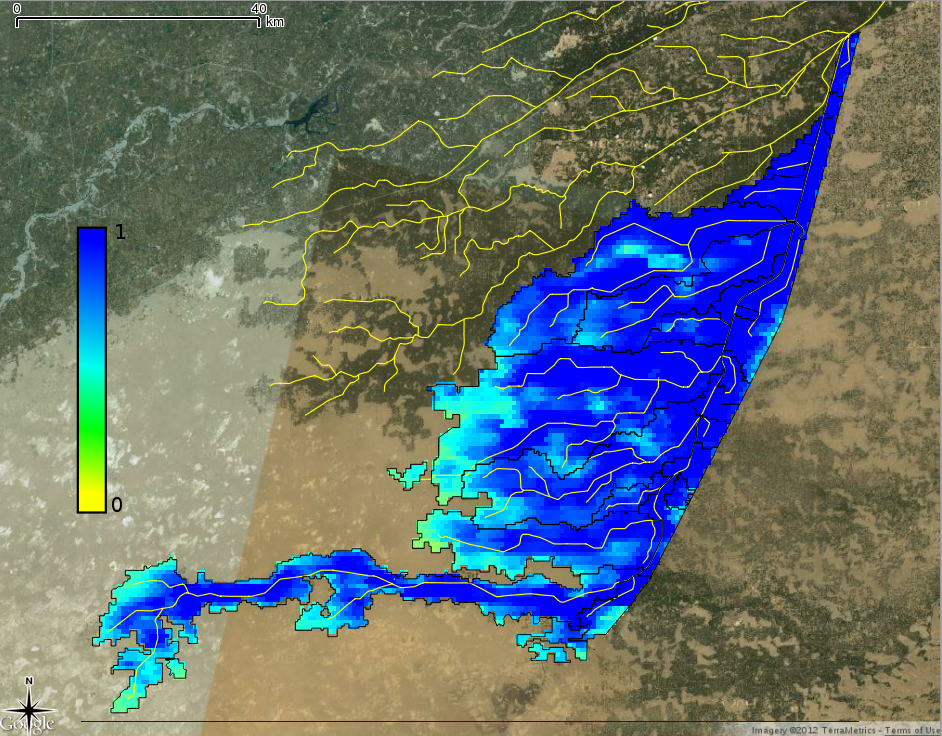
\includegraphics[width=4cm]{fess2012ef}
\end{center}

\column{0.8\textwidth}
\begin{flushright}
  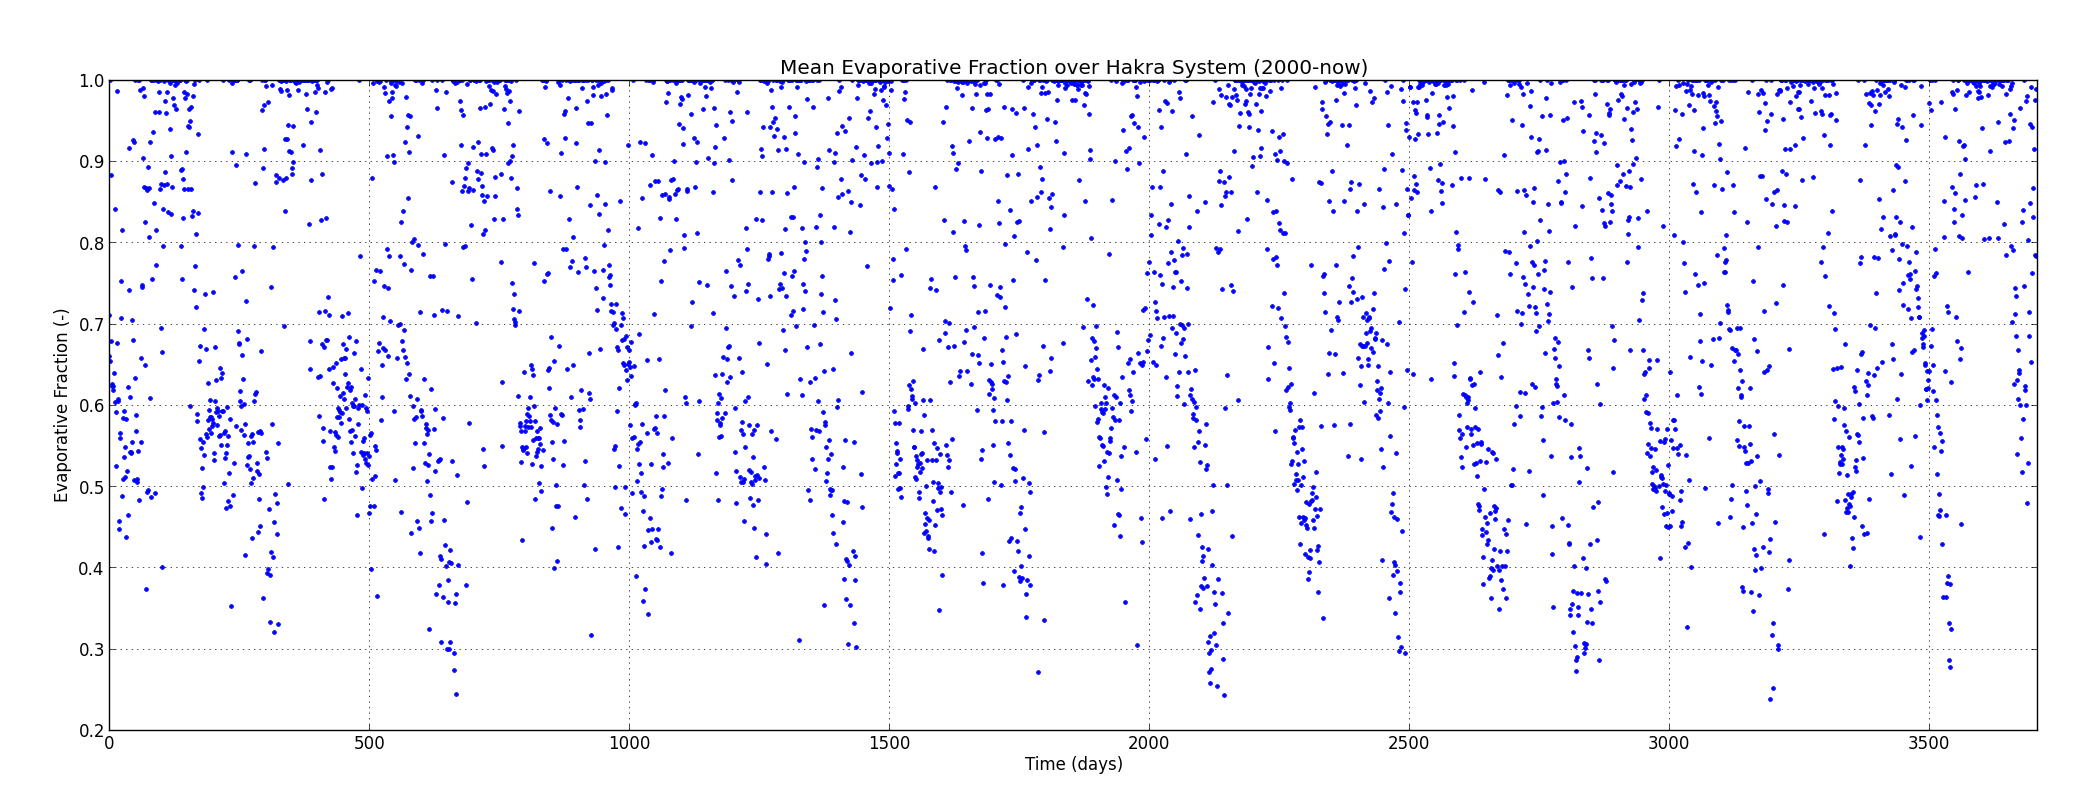
\includegraphics[width=8cm]{fess2012meaneftemporal}
\end{flushright}
\end{columns}

\end{frame}

%%%%%%%%%%%%%%%%%%%%%%%%%%%%%%%%%%%%%%%%%%%%%%%%%%%%%%%%%%%%%%%%%%%%
\begin{frame}[fragile]{Crop water consumption in irrigation systems}

Actual evapotranspiration (mm/d, daily, 11 years)\\ 
for agricultural water performance management.\\

\begin{center}
 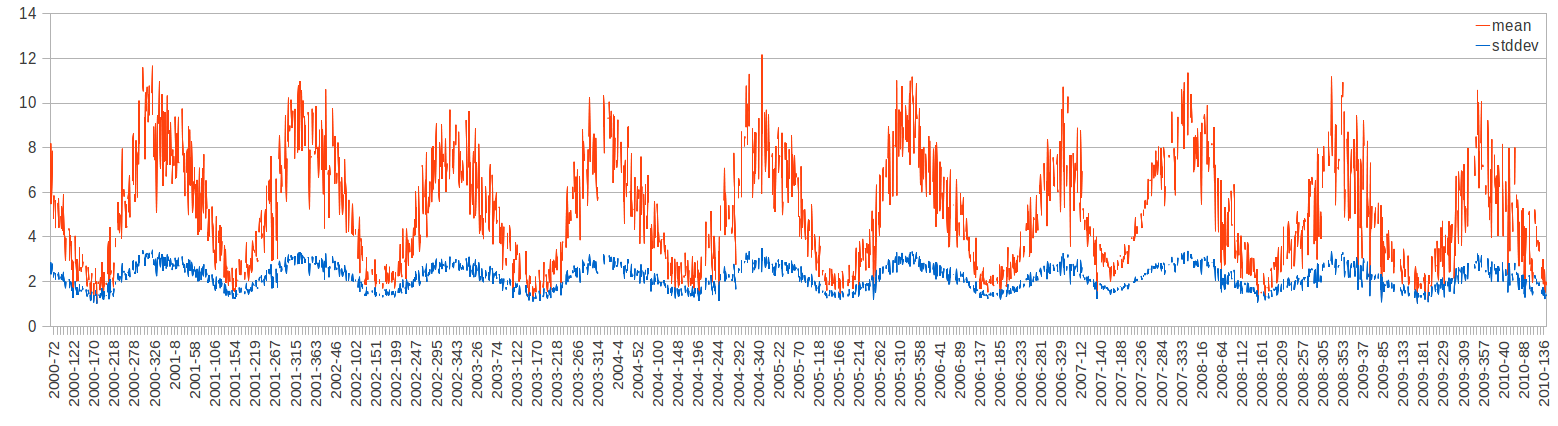
\includegraphics[width=9.5cm]{ciameanet}\\
 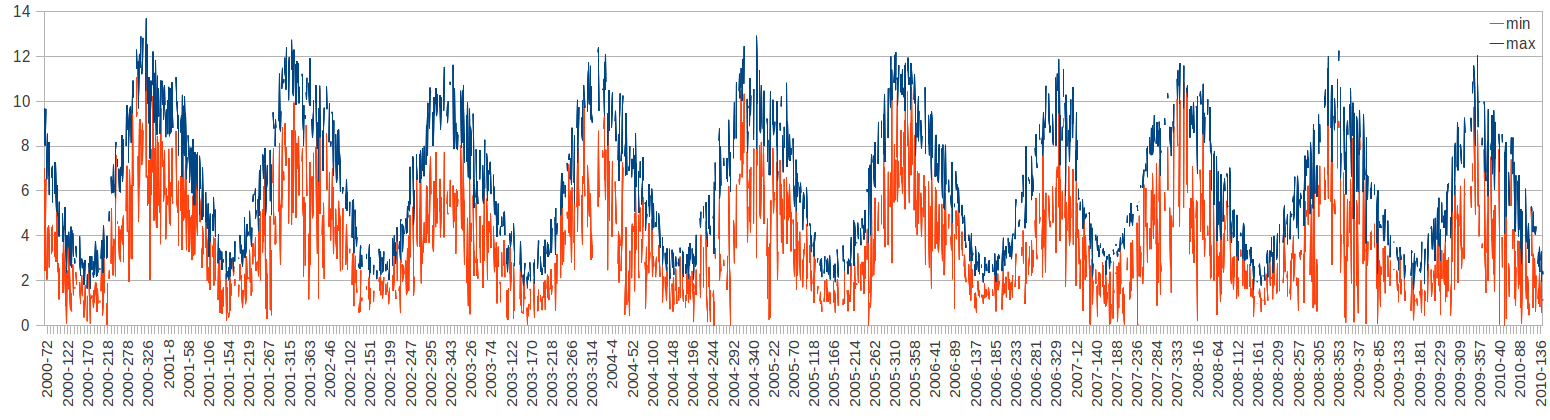
\includegraphics[width=9.5cm]{ciaminmaxet}
\end{center}

\end{frame}

\section{Frameworks}
\subsection{Chain processing}
%%%%%%%%%%%%%%%%%%%%%%%%%%%%%%%%%%%%%%%%%%%%%%%%%%%%%%%%%%%%%%%%%%%%
\begin{frame}[fragile]{Chain processing}

Chain processing has a fundamental impact on remote sensing work:\\

\begin{itemize}
 \item Standardization limits bugs
 \item Less prone to human error
 \item Simpler parameterization access
 \item Permits to apply any number of modules to all target images
 \item Ensures maximum quality of generated images
\end{itemize}

\end{frame}

\subsection{Blueprint}
%%%%%%%%%%%%%%%%%%%%%%%%%%%%%%%%%%%%%%%%%%%%%%%%%%%%%%%%%%%%%%%%%%%%
\begin{frame}[fragile]{Blueprint}

\begin{center}
 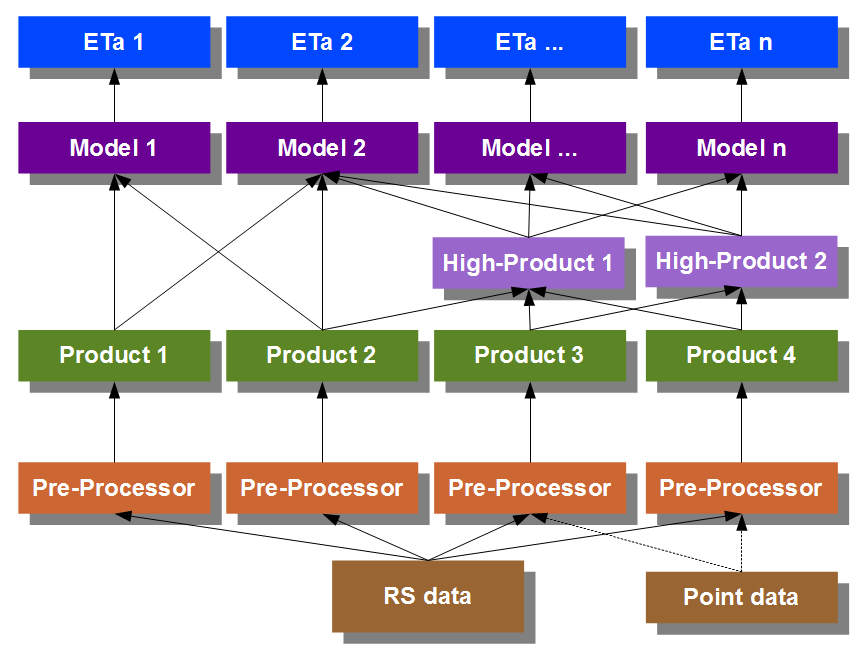
\includegraphics[width=7.5cm]{chain0}
\end{center}

\begin{itemize}
 \item GDAL+[C+OpenMP]
 \item GRASSGIS+pyGRASS+[C+OpenMP]
\end{itemize}

\end{frame}

\subsection{GDAL}
%%%%%%%%%%%%%%%%%%%%%%%%%%%%%%%%%%%%%%%%%%%%%%%%%%%%%%%%%%%%%%%%%%%%
\begin{frame}[fragile]{GDAL framework}

\begin{columns}[l]
\column[t]{0.6\textwidth}
\begin{center}
 GDAL+[C+OpenMP]
 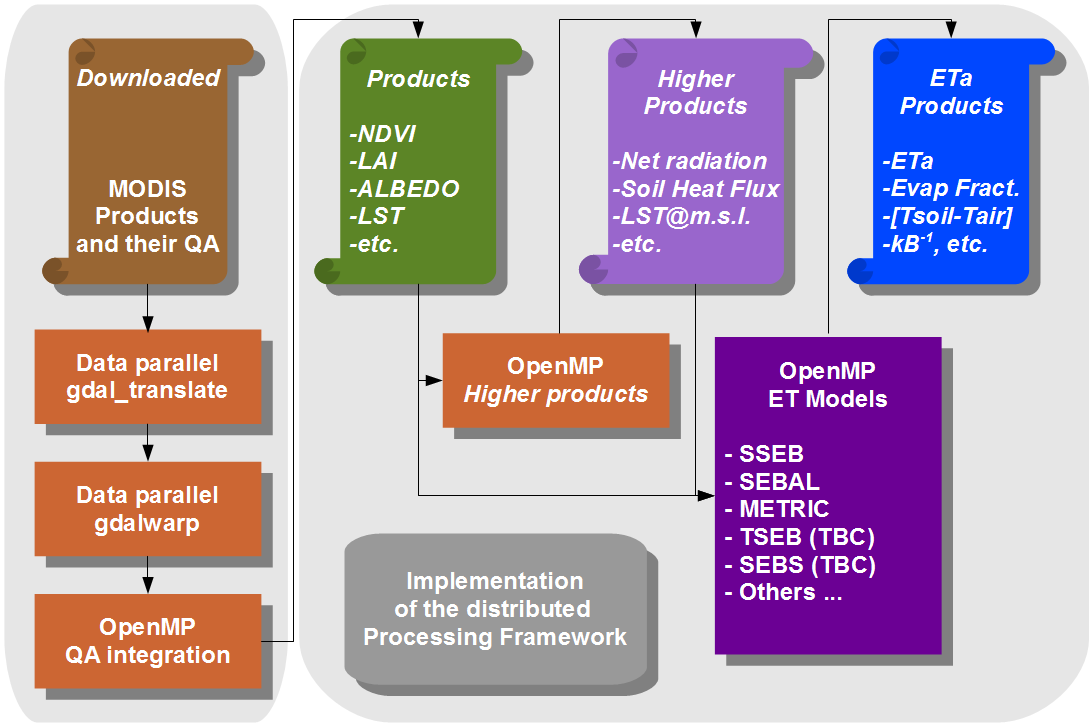
\includegraphics[width=7.5cm]{chain2}
\end{center}
\column[t]{0.4\textwidth}
\begin{center}
 OpenMP distribution
 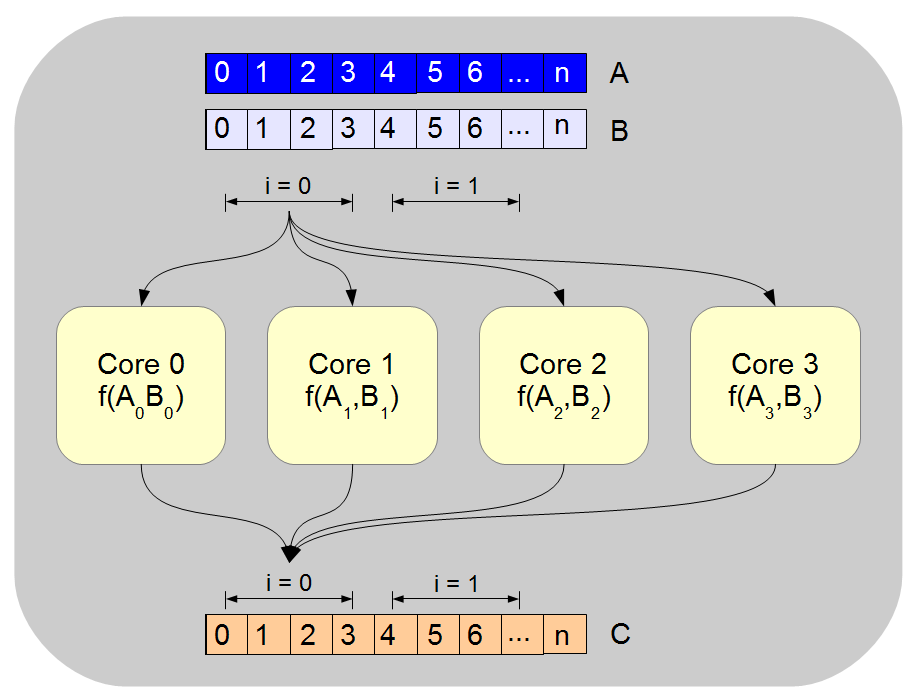
\includegraphics[width=5cm]{chain1}
\end{center}
\end{columns}
\end{frame}


\subsection{GRASS GIS}
%%%%%%%%%%%%%%%%%%%%%%%%%%%%%%%%%%%%%%%%%%%%%%%%%%%%%%%%%%%%%%%%%%%%
\begin{frame}[fragile]{GRASS GIS framework}

\begin{center}
 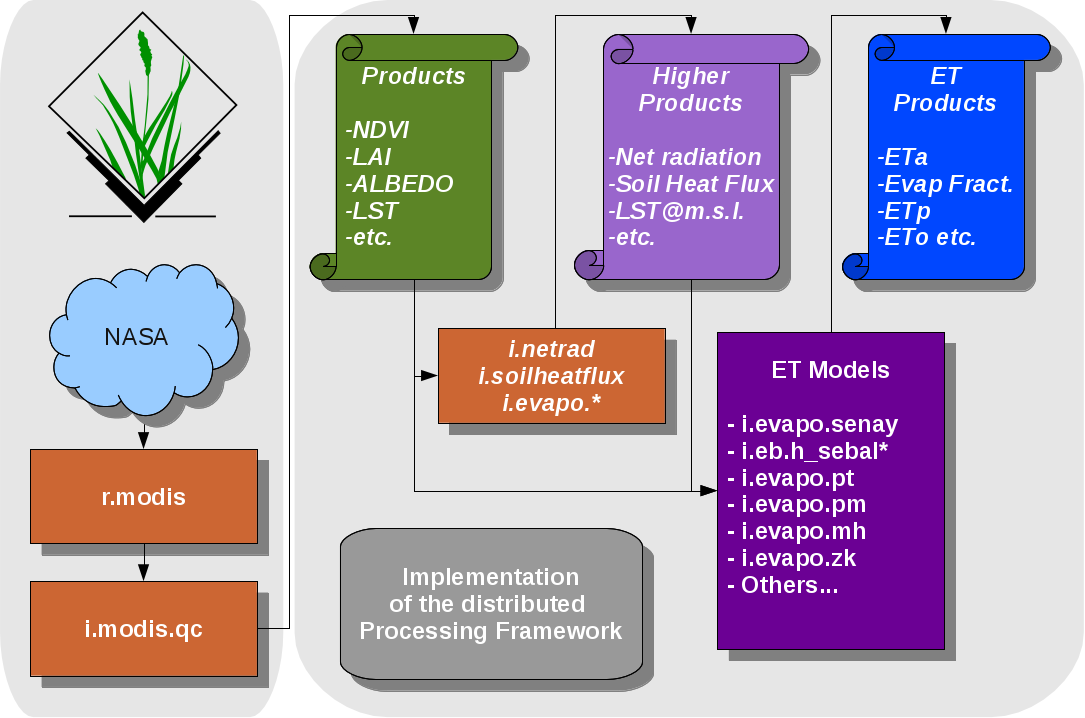
\includegraphics[width=7.5cm]{architecture_implementation}
\end{center}

\begin{block}{metaModule concept}
{\bf pyGRASS:} vertical integration of GRASS GIS modules\\
{\bf GRASS GIS modules:} [C+OpenMP]
\end{block}

\end{frame}

\section{Initial results}
%%%%%%%%%%%%%%%%%%%%%%%%%%%%%%%%%%%%%%%%%%%%%%%%%%%%%%%%%%%%%%%%%%%%
\begin{frame}[fragile]{Initial results}

\begin{center}
 Average ET for Sri Lanka, Daily 2000-2012 (mm/d, daily, 12.3 years)
 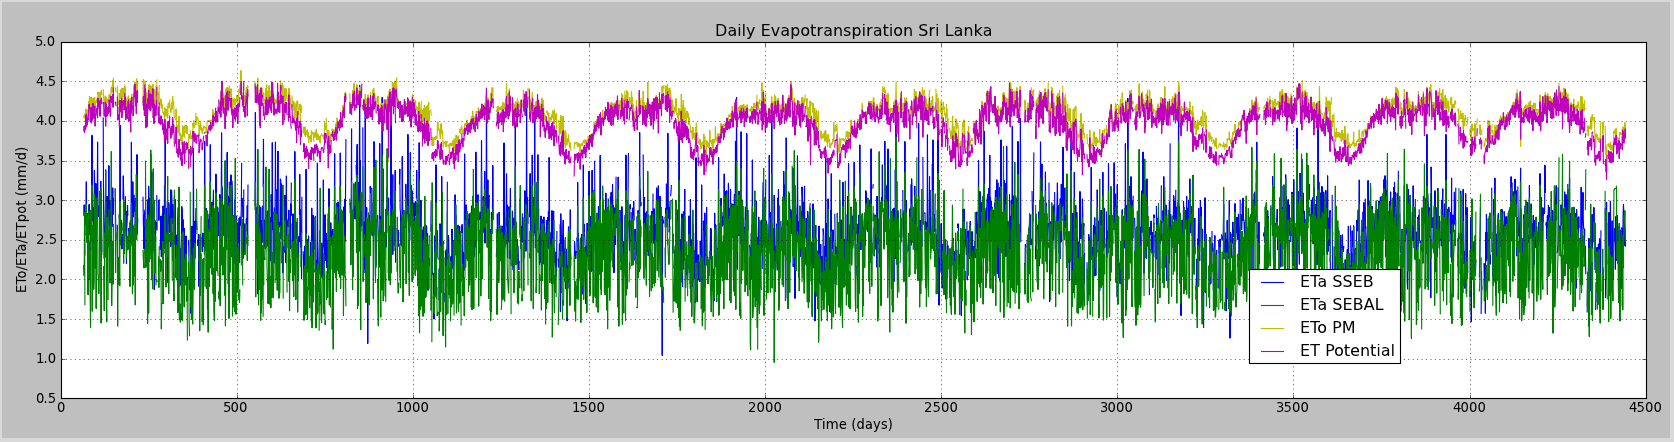
\includegraphics[width=12cm]{sltemporaletb}
\end{center}

\begin{block}{Comparison}
\begin{itemize}
 \item ETo \& ETpot (rad) are similar, expected.
 \item ETa models are not so similar, expected.
 \item ETo \& ETpot (rad) are higher than ETa models, expected.
\end{itemize}

\end{block}

\end{frame}

\section{Conclusions}
%%%%%%%%%%%%%%%%%%%%%%%%%%%%%%%%%%%%%%%%%%%%%%%%%%%%%%%%%%%%%%%%%%%%
\begin{frame}[fragile]{Conclusions}

\begin{block}{Distributed ET models benchmarking setup with OSGEO tools}
\begin{itemize}
 \item {\bf GDAL:} C+OpenMP, core-based scaling
 \item {\bf GRASS GIS:} pyGRASS for metaModule, C+OpenMP inside modules
 \item {\bf Targets (1):} MODIS (Terra/Aqua), Landsat (all), Aster
 \item Points of comparisons are internal and main outputs
\end{itemize}
\end{block}

\end{frame}

%%%%%%%%%%%%%%%%%%%%%%%%%%%%%%%%%%%%%%%%%%%%%%%%%%%%%%%%%%%%%%%%%%%%
\begin{frame}[fragile]{Thank You}

\begin{center}
 
\includegraphics[width=3cm]{OpenInnovation}
\end{center}

\end{frame}

%%%%%%%%%%%%%%%%%%%%%%%%%%%%%%%%%%%%%%%%%%%%%%%%%%%%%%%%%%%%%%%%%%%%
\begin{frame}[fragile]{Outlooks}

\begin{itemize}
 \item {\bf Crunch (1):} Multi-GPU distribution (OpenCL, CUDA)
 \item {\bf Crunch (2):} Multi-CPU distribution (MPI)
 \item {\bf Think (1):} TSEB to test/fix
 \item {\bf Think (2):} SEBS to complete
 \item {\bf More (1):} ETLook to digest and code
 \item {\bf More (2):} MODIS and Landsat archives under close pipe distance?
\end{itemize}

\end{frame}

%%%%%%%%%%%%%%%%%%%%%%%%%%%%%%%%%%%%%%%%%%%%%%%%%%%%%%%%%%%%%%%%%%%%
\begin{frame}[fragile]{128-cores Tilera}

\begin{columns}[l]
\column[t]{0.5\textwidth}
\begin{center}
 64-core Tile-GX\newline\linebreak
 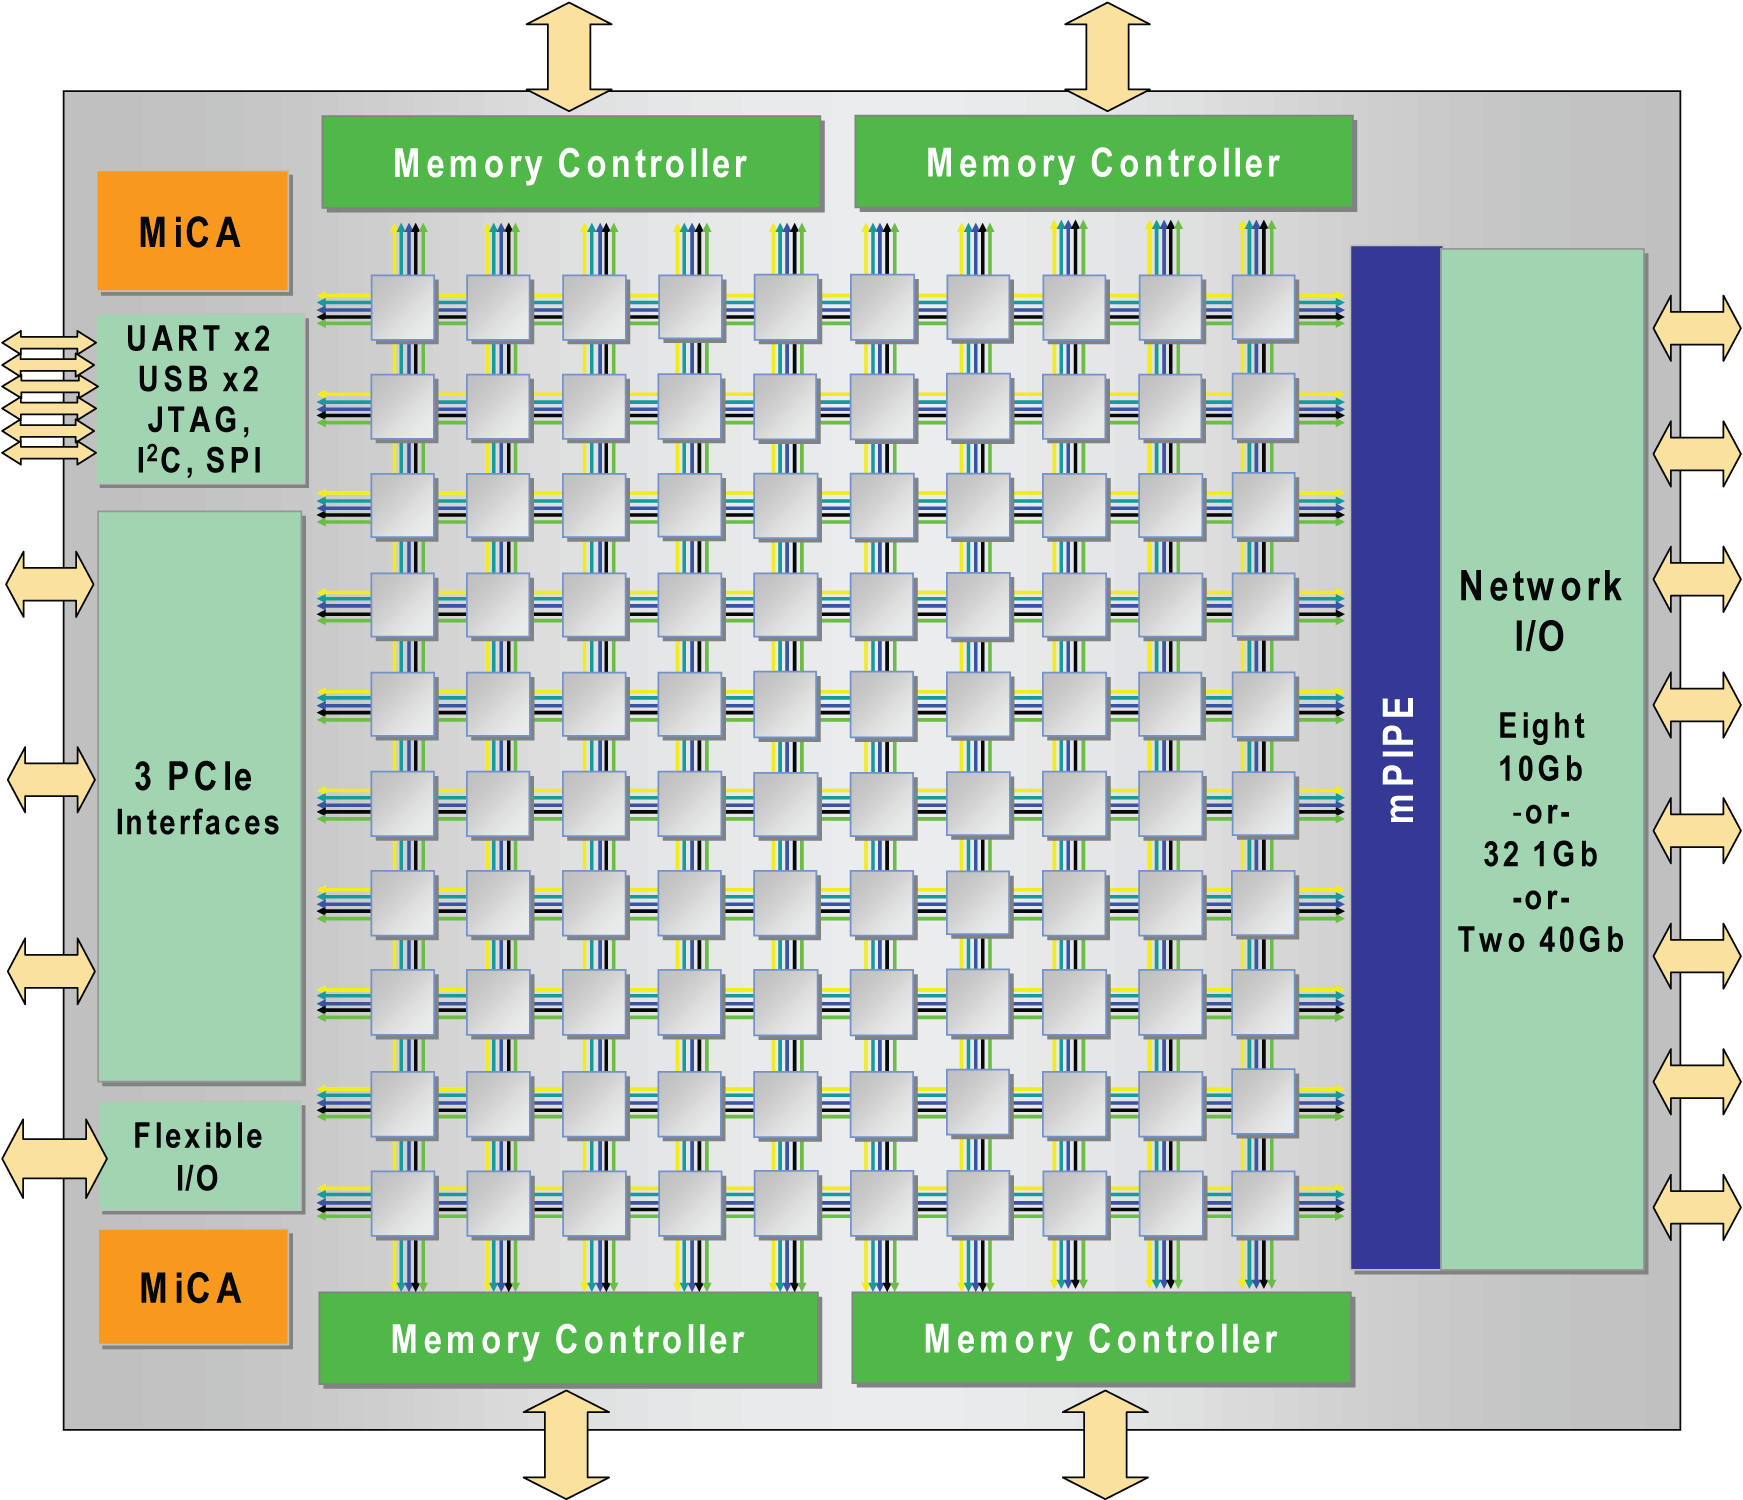
\includegraphics[width=5cm]{TILE-Gx_Block_Diagram_large}
\end{center}
\column[t]{0.5\textwidth}
\begin{center}
 Dual Tile-GX on {\small $1/2$} rack board\newline\linebreak
 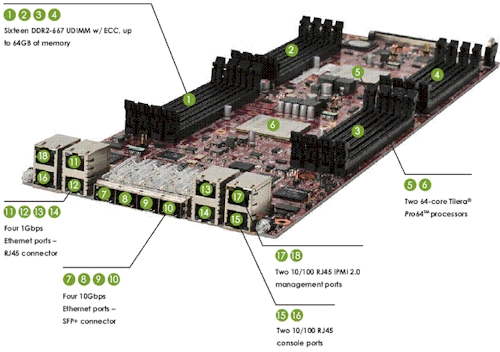
\includegraphics[width=5cm]{tilera_quanta_sq2_mobo}
\end{center}

\end{columns}

\end{frame}

\end{document}
